\Lecture{Jayalal Sarma}{Sept 19, 2020}{05}{Multichoosing}{Narasimha Sai Vempati}{$\alpha$}{JS}

\section{Introduction}
Consider the definition of \emph{set}. We know that it's a well defined collection of \emph{distinct} objects. From a collection of $n$ distinct symbols, the number of ways to form a \emph{set} of length $k$ is given by $\binom{n}{k}$. Now let's consider the definition of \emph{multi-set}. It's similar to that of a \emph{set}, except that it allows repetition of objects. Now it's natural ask the following question: From a collection of $n$ distinct symbols, what is the number of ways to form a \emph{multi-set} of length $k$. Multichoosing exactly answers this questions. In this lecture, we explore multichoosing in detail. We discuss several equivalent bijections to this problem and come-up with an algebraic expression for \mulnom{n}{k} (spelled out as $n$ \emph{multi-choose} $k$).

\section{Equivalent bijections} \label{sec:equi-bij}
\subsection{Non-negative solutions}\label{non-neq-sol-prob}
Formally, \mulnom{n}{k} is the number of ways of choosing $k$ objects from a set of $n$ objects where the order is not important but repetitions are allowed. For all $i=1,2,\cdots,n$, if we denote by $x_i$ the number of copies of $i^{th}$ object we choose, then we have the equation \begin{equation}\label{eqn1}
    x_1+x_2+\cdots+x_n=k
\end{equation} where each $x_i \geq 0$. Therefore, number of \emph{non-negative} integral solutions to this equation gives us the required number of ways of choosing $k$ objects from $n$ objects with given conditions. Let's look at an equivalent problem and establish a bijection between these two.

\subsection{Voting problem}\label{voting-prob} If $n$ candidates are contesting in an election and there are $k$ voters, how many ways can votes of those $k$ voters be distributed among $n$ candidates? 

If we denote by $x_i$, the number of votes received by $i^{th}$ candidate and there are $k$ voters, we have $x_1+x_2+\cdots+x_n=k$ and thus, the number of ways of dividing votes among candidates is the number of non-negative solutions to the equation \ref{eqn1}. Formally, we can define a bijection $f$ from set of solutions to the equation \ref{eqn1} to set of ways of dividing the votes among $n$ candidates. 
\begin{description}
\item\underline{Definition:}  $f$ takes the tuple $\vecx=(x_1,x_2,\cdots,x_n)$ and assign $x_i$ number of votes to $i^{th}$ candidate where $i=1,2,\cdots,n$.
\item\underline{Well defined:} $f$ is well defined because for every valid tuple $\vecx=(x_1,x_2,\cdots,x_n)$, we have $x_1+\cdots+x_n=k$ and thus summing over votes received by $i^{th}$ where $i=1,2,\cdots,n$ will be $k$ votes in total. 
%there is a unique way of dividing the votes among candidates. In other words, for any two distinct way of dividing $k$ votes among $n$ candidates, there must exists an $i$ such that number of votes received $i^{th}$ candidate is different and thus $x_{1_i} \neq x_{2_i}$. Therefore $\vecx_1\neq\vecx_2$. 
\item\underline{Injective:} $f$ is an injection because for every valid way of dividing the votes among candidates, there's a unique solution tuple in which $x_i = $ number of votes received by $i^{th}$ candidate. In other words, for any two $\vecx_1\neq\vecx_2$, there exists an $i\in[n]$ such that $x_{1_i}\neq x_{2_i}$ and $i^{th}$ candidate gets different votes. Thus $f(\vecx_1)\neq f(\vecx_2)$.
\item\underline{Surjective:} $f$ is surjective because for every way of dividing $k$ votes among $n$ candidates, there is a pre-image $\vecx=(x_1,\cdots,x_n)$ which is a valid solution to the equation \ref{eqn1} (as there are a total of $k$ voters, sum of number of votes received by each voter must sum up to $k$). 
\end{description}
Thus $f$ is a bijection from the set of non-negative solutions to $x_1+\cdots+x_n=k$ to the set of ways of dividing $k$ votes among $n$ candidates.
\subsection{Non-decreasing subsequences}\label{non-dec-subseq-prob} Number of non-decreasing sequences of integers between $1$ and $n$ of length $k$. A non-decreasing sequence is of the form $\{a_1,a_2,\cdots,a_k\}$ where $1\leq a_1\leq a_2\cdots\leq a_k\leq n$. Lets define a bijection $f$ from set of non-negative integral solutions to Eqn. \ref{eqn1} to set of non-decreasing sequences between $1$ and $n$ of length $k$. 
\begin{description}
\item\underline{Definition:} $f$ takes $\vecx=(x_1,\cdots,x_n)$ as input and writes the number $i$ $x_i$ times for all $i=1,2,\cdots,n$ to obtain a sequence of length $k$.
\item\underline{Well defined:} As $f$ constructs the sequence in increasing order from $1$ to $n$ by writing $i$ $x_i$ times, the resulting sequence will be non-decreasing. Therefore, $f$ is well defined.
\item\underline{Injective:} For every $\vecx_1\neq\vecx_2$, there exists an $i$ such that $x_{1_i} \neq x_{2_i}$ and thus in the resulting sequences, number $i$ is written different number of times. Therefore, $f$ is injective.
\item\underline{Surjective:} Every non-decreasing sequence of integers between $1$ and $n$ of length $k$ has a pre-image $\vecx=(x_1,\cdots,x_n)$  which is a valid solution to equation \ref{eqn1} (where $x_i$ is the number of times the number $i$ is present in the sequence and as length of sequence is $k$, all $x_i$'s where $i=1,2,\cdots,n$ sum up to $k$).
\end{description}
Thus $f$ is a bijection.
\subsection{Stars and bars problem}\label{star-bar-prob} There are $k$ stars placed horizontally. Find the number of ways to place $n-1$ bars in between those $k$ stars. Lets define a bijection $f$ from set of non-negative integral solutions to Eqn. \ref{eqn1} to set of ways of placing $n-1$ bars among $k$ stars.
\begin{description}
\item\underline{Definition:} $f$ takes $\vecx=(x_1,\cdots,x_n)$ as input and place $x_i$ number of stars between $(i-1)^{th}$ bar and $i^{th}$ bar. We leave it as an exercise to prove that $f$ is well-defined, injective and surjective.
\end{description}
\jsay{Prove that $f$ is a bijection}

\section{Algebraic expression}\label{alg-expr}
So far in Sec. \ref{sec:equi-bij}, we have established bijections between \emph{non-negatives integral} solutions of Eq. \ref{eqn1} and various other problems and argued that number of ways of solving any particular problem is equal to the number of non-negative integral solutions to Eq. \ref{eqn1}. In this section, we are interested in coming up with a concrete expression for \mulnom{n}{k} by solving it's equivalent bijection.

\paragraph{Method 1} Let's solve the \emph{stars and bars} problem defined in Sec. \ref{star-bar-prob}. Let's use the fact that any placement of $n-1$ bars among $k$ stars can be equivalently thought of as a string of length $n+k-1$ over the alphabet $\{\star,|\}$ with $k$ $\star$'s. Therefore, \begin{align*}
    \textrm{number of ways of placing } n-1 \textrm{ bars among } k \textrm{ stars } &= \textrm{number of such strings}\\
    &= \binom{n+k-1}{k}
\end{align*}

\paragraph{Method 2} Let's solve the \emph{Non-decreasing subsequences} problem defined in Sec. \ref{non-neq-sol-prob}. Let's establish a bijection $f$ from set $\beta$ of non-decreasing subsequences of integers between $1$ and $n$ of length $k$ to a set $\Gamma$ of strictly increasing subsequences of integers between $1$ and $n+k-1$ of length $k$. A strictly increasing subsequence is of the form $1\leq b_1<b_2<\cdots<b_k\leq n+k-1$
\begin{description}
\item{\underline{Definition:}} $f$ takes as input a non-decreasing subsequence $(a_1,a_2,\cdots,a_k)$ between $1$ and $n$ and for all $i=1,2,\cdots,k$ set $b_i = a_i+i-1$ and output the sequence $(b_1,b_2,\cdots,b_k)$
\item{\underline{Well defined:}} For any $(a_1,a_2,\cdots,a_k)\in\beta$, we have for all $i=1,2,\cdots,k-1$, \begin{align*}
    a_i &\leq a_{i+1}\\
    a_i+i &\leq a_{i+1}+i\\
    a_i+i-1 &< a_{i+1}+i\\
    b_i &< b_{i+1}
\end{align*}  Therefore, the subsequence $(b_1,\cdots,b_k)$ is strictly increasing subsequence and thus $f$ is well defined.
\item{\underline{Injective:}} For every non-decreasing subsequence $(a_1,\cdots,a_k)$, there's a unique strictly increasing subsequence $(b_1,\cdots,b_k)$ where for all $i=1,\cdots,k$, $b_i = a_i+i-1$. Therefore $f$ is injective.
\item{\underline{Surjective:}} For every strictly increasing subsequence $(b_1,\cdots,b_k)$, there's a pre-image $(a_1,\cdots,a_k)$ which is non-decreasing where for all $i=1,\cdots,k$, $a_i=b_i-i+1$
\end{description}


Therefore, $f$ is a bijection. The number of ways of choosing a strictly increasing subsequence $(b_1,\cdots,b_k)$ between integers $1$ and $n+k-1$ is just choosing $k$ integers from first $n+k-1$ integers and arrange them in one way(increasing order). Therefore number of ways = $\binom{n+k-1}{k}$. As $f$ is a bijection, therefore, the number of non-decreasing subsequences between $1$ and $n$ of length $k$ are $\binom{n+k-1}{k}$

\paragraph{Method 3} Let's solve the \emph{Voting} problem defined in Sec. \ref{voting-prob}. Let's ask a slightly modified question. 
\begin{description}
\item \underline{Question:} How many ways to distribute $m$ votes among $n$ candidates such that each candidate gets at least one vote.
\item \underline{Answer 1:} As every candidate gets at least one vote, let's first distribute one vote each to each of the $n$ candidate and the distribute the remaining $m-n$ votes among $n$ candidates. By the bijection defined in Sec. \ref{voting-prob}, the number of ways of distributing $m-n$ votes among $n$ candidates is \mulnom{n}{m-n}  
\item \underline{Answer 2:} Let's interpret votes as $\star$ s. Then the question essentially reduces to placing $n-1$ bars (since there are $n$ candidates, we divide by placing $n-1$ bars) among $m$ stars (since there are $m$ voters). $i^{th}$ candidate gets votes equal to number of stars between $(i-1)^{th}~|$ and $i^{th}~|$. However, there are two additional constraints \begin{enumerate}
    \item\label{cond1} A bar cannot be placed in the beginning or in the end (if not then either the first candidate or the last candidate gets $0$ votes)
    \item\label{cond2} We cannot place two $|$ s between same two $\star$ s (if we place $(i-1)^{th}~|$ and $i^{th}~|$ between same two $\star$ s, the $i^{th}$ candidate gets $0$ votes)
\end{enumerate}
Hence, we have to choose $n-1$ gaps among the $m-1$ gaps (because we have $m+1$ gaps and by cond. \ref{cond1} we remove two) to place $n-1~|$ s without repetitions (because repeating violates cond. \ref{cond2}). Therefore, there are $\binom{m-1}{n-1}$ ways of doing it. Thus \mulnom{n}{m-n}=$\binom{m-1}{n-1}$ and by substituting $m=n+k$, we have $$\textrm{\mulnom{n}{k}}=\binom{n+k-1}{n-1}=\binom{n+k-1}{k}$$
\end{description}
\section{Identities}
In this section, we discuss some identities on \mulnom{n}{k} and argue their proofs using the idea of either double counting or bijections.
\paragraph{Identity 1} $$\textrm{\mulnom{n}{k}}=\textrm{\mulnom{k+1}{n-1}}$$
\begin{proof}
Let's use the bijection method to prove this. Formally, lets define sets $S_1$ and $S_2$ and count their cardinalities independently and then establish a bijection from $S_1$ to $S_2$ proving that $|S_1|=|S_2|$.
\begin{description}
\item \underline{$S_1$:} Configuration of $k~\star$ s and $n-1~|$ s as described in Sec. \ref{star-bar-prob}. By the bijection defined in it, $|S_1|=$ \mulnom{n}{k}
\item \underline{$S_2$:} Configuration of $n-1~\star$ s and $k~|$ s as described in Sec. \ref{star-bar-prob}. Again, by the bijection defined in it, $|S_2|=$\mulnom{k+1}{n-1}
\item \underline{Bijection:} Let's define a bijection $f$ from $S_1$ to $S_2$. $f$ takes a configuration from $S_1$ as input and interpret $\star$ s as $|$ s and $|$ s as $\star$ s. Therefore it ends up with a configuration with $n-1~\star$ s and $k~|$ s which is a configuration is $S_2$. It's easy to observe that $f$ is a bijection.
\end{description}
As $f$ is a bijection from $S_1$ to $S_2$, we have $|S_1|=|S_2|$. This completes the proof 
\end{proof}

\paragraph{Identity 2}
$$k~\textrm{\mulnom{n}{k}}=n~\textrm{\mulnom{n+1}{k-1}}$$
\begin{proof}
Let's use the method of double counting to prove this.
\begin{description}
\item \underline{Question:} In how many ways can we construct a non-decreasing sequence $1\leq a_1\leq a_2\cdots\leq a_k\leq n$ and mark one element?
\item \underline{Asnwer 1:} By the bijection established in Sec. \ref{non-dec-subseq-prob} we have \mulnom{n}{k} number of non-decreasing subsequences and for every such subsequence, we can mark any one of the $k$ elements choose. Thus the answer is $k$ \mulnom{n}{k} 
\item \underline{Answer 2:} Firstly, determine the value in $[n]$ which is to be marked. Let $r$ be this value. Now, consider a non-decreasing subsequence between $1$ and $n+1$ with $k-1$ elements. Using $r$ and the non-decreasing sequence chosen, we construct a unique non-decreasing sequence between $1$ and $n$ of length $k$ with $r$ as marked in the following way:

Let $(b_1,b_2,\cdots,b_{k-1})$ with $1\leq b_1\leq b_2\leq\cdots\leq b_{k-1}\leq n+1$ be the chosen sequence, 
\begin{itemize}
    \item Insert marked-$r$ in the right most position so that the resulting sequence is still sorted.
    \item As long as there's an $n+1$ in the sequence, remove it and add it as $r$ to the right of marked-$r$ in the sequence
\end{itemize}
Therefore, number of required sequences 
\begin{align*}
    &= \textrm{ number of ways to choose }r \times \substack{\textrm{ number of non-decreasing sequences of length }\\ k-1 \textrm{ between } 1 \textrm{ and } n+1}\\
    &= n\times \textrm{\mulnom{n+1}{k-1}}
\end{align*}
\end{description}
This completes the proof
\end{proof}

\begin{ex}
    \item Prove the following by combinatorial arguments $$\textrm{\mulnom{n}{k}}=\sum\limits_{m=1}^{n}\textrm{\mulnom{m}{k-1}}$$ \emph{Hint: Look for bijection to number of non-decreasing subsequences}
    \item Prove the following by combinatorial arguments $$\sum\limits_{k=0}^{m}\textrm{\mulnom{n}{k}}=\textrm{\mulnom{n+1}{m}}$$ \emph{Hint: Look for bijection to Voting problem}
    \item Prove the following by combinatorial arguments $$\textrm{\mulnom{n}{k}}=\sum\limits_{m=0}^{n}\binom{n}{m}\textrm{\mulnom{m}{k-m}}$$
\end{ex}

\Lecture{Jayalal Sarma}{Sept 19, 2020}{06}{Catlan Bijections}{Anshu and Narasimha Sai}{$\alpha$}{JS}

\section{Introduction}
One of the classic examples to demonstrate the power of bijections is \emph{Catlan numbers}. The Catlan numbers form a sequence of natural numbers that occur in various counting problems and occurs in several seemingly different contexts. Historically, \emph{Euler} is the first person to study them. He was interested in counting the number of ways of dividing a polygon into triangles by drawing non-overlapping diagonals. Catlan numbers got their name from \emph{Eugene Catlan} when he used them to answer the \emph{Parenthesisation problem} which is the following: Consider a sequence $(a_1,a_2,\cdots,a_{n+1})$ of $n+1$ numbers, If we have to perform a binary operations $\odot$ $n$ times among them, how many number of ways are there to parenthesise (or bracket) them using $n$ parenthesis of single type (say $'()'$). In this lecture, we will see a few equivalent problems to this and then arrive at an explicit expression of Catlan numbers.
\section{Equivalent Bijections}
In this section, we see a few equivalent problems of the \emph{parenthesisation} problem and argue that answer to each of them is also the \emph{catlan number}
\paragraph{Full binary trees} If we observe the Parenthesisation problem carefully, we notice that every valid parentesisation of those $n+1$ numbers form a \emph{full binary tree} (a binary tree in which every node have either two children or no children) of $n+1$ leaves and $n$ internal nodes where leaves represents the numbers $a_1,\cdots,a_{n+1}$ and each internal node corresponds to one operation. Therefore, there's an implicit bijection between the set of valid parenthesisations and full binary trees with $n$ internal nodes. Therefore, 
\begin{equation}
    \substack{\textrm{number of valid parenthesisations of }\\ n+1 \textrm{ elements }}  = \substack{\textrm{number of full binary trees with }\\ n \textrm{ internal nodes}}
\end{equation}  

\paragraph{Balanced parenthesised strings} A balanced parenthesised string of length $2n$ is a string consists of $n$ left brackets $'('$ and $n$ right brackets $')'$ in which every prefix of the string has number of left brackets $'('$ $\geq$ number of right brackets $')'$. One can easily observe the bijection from set of balanced paranthesised string to valid parenthesisations of $n+1$ numbers

\paragraph{Euler's problem} Find the number of ways of triangulating a polygon with $n+2$ edges

\paragraph{Handshaking problem} Consider a scenario where $2n$ people are sitting around a table. How many ways they can shake hands with each other without crossing hands. We leave it as an exercise to establish bijections from \emph{Euler's} problem to \emph{Full binary tree} problem and \emph{handshaking} problem to \emph{balanced parenthesised strings} problem.
\jsay{Establish bijections from \emph{Euler's} problem to \emph{Full binary tree} problem and \emph{handshaking} problem to \emph{balanced parenthesised strings} problem}

\section{Algebraic Expression}
In this section, we are interested in arriving at a concrete expression of the $n^{th}$ \emph{catlan number} (denoted by $c_n$). Let's solve another problem and then, by establishing a bijection to one of the above problems, we can arrive at an expression for $c_n$.

\subsection{Monotone walk on $n\times n$ grid} Suppose we have a grid of size $n\times n$. How many ways are there to go from $(0,0)$ to $(n,n)$ by using only downward edges or right edges. A sample path is represented in Fig. \ref{fig:sample-path}. We observe that each step can increment the value of exactly one of the co-ordinates by $1$. Since we have to move from $(0,0)$ to $(n,n)$, we have to increase the value of both the co-ordinates by $n$ and $n$ and thus irrespective of the path you take, the length of a path from $(0,0)$ to $(n,n)$ must be of length $n+n=2n$.

\begin{figure}[h!]
    \centering
    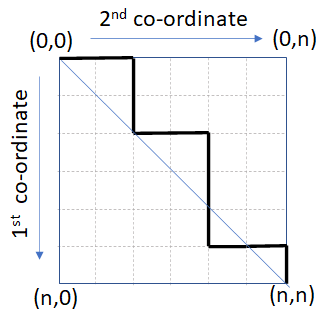
\includegraphics[width=0.4\linewidth]{images/sample-path.png}
    \caption{A path from $(0,0)$ to $(n,n)$ using downward and right edges}
    \label{fig:sample-path}
\end{figure}

If we represent each right move as $R$ and each downward move as $D$, one can observe that there's a bijection $f$ from the set of paths to set of strings of length $2n$ over the alphabet $\{D,R\}$ with number of $D$'s = number of $R$'s = $n$. Formally, if $(u_0,v_0), (u_1,v_1),\cdots,(u_{2n},v_{2n})$ represents the path where $(u_0,v_0)=(0,0)$ and $(u_{2n},v_{2n})=(n,n)$, and $b=b_1b_2\cdots b_{2n}$ represents the string where each $b_i$ is either $D$ or $R$, our bijection $f$ takes a path as input and sets $b_i$ as
$$b_i=\begin{cases}
D &\mbox{if } u_i = u_{i-1}+1\\
R &\mbox{if } v_i = v_{i-1}+1
\end{cases}$$
\begin{description}
\item \underline{Well defined:} As we have exactly $n$ $x$ co-ordinate increments and $n$ $y$ co-ordinate increments, we will have exactly $n$ $D$'s and $n$ $R$'s in our string and thus $f$ is well defined.
\item \underline{Injective:} Two different paths from $(0,0)$ to $(n,n)$ will different in at least one $(u_{i-1},v_{i-1})$ to $(u_i,v_i)$ transition where $i=1,2,\cdots,2n$, their corresponding strings under $f$ will differ in at least $i^{th}$ position and thus $f$ is injective.
\item \underline{Surjective:} Every string over $\{D,R\}$ of length $2n$ with equal number of $D$'s and $R$'s has a pre-image under $f$ which is defined by $(u_0,v_0)=(0,0)$ and $(u_i,v_i)$ is $(u_{i-1}+1,v_{i-1})$ if $b_i=R$ and $(u_{i-1},v_{i-1}+1)$ if $b_i=D$. As there will be $n$ $D$'s and $n$ $R$'s, $(u_{2n},v_{2n})=(n,n)$ and thus $f$ is surjective .
\end{description} 
Thus $f$ is bijection. As we have number of string over $\{D,R\}$ of length $2n$ with equal number of $D$'s and $R$'s equal to $\binom{2n}{n}$ (select $n$ positions out of $2n$ available and fill them with $D$'s and the rest with $R$'s). Thus the number of paths from $(0,0)$ to $(n,n)$ with only downward and rightward movements is $\binom{2n}{n}$.

Lets ask a slightly question. How many ways are there to go from $(0,0)$ to $(n+1,n-1)$ using only downward or right edges.Using a similar arguments as above, we can come up with a bijection to set of string over $\{D,R\}$ of length $2n$ with $n+1$ $D$'s and $n-1$ $R$'s. Therefore number of required paths are $\binom{2n}{n+1}=\binom{2n}{n-1}$

%\Lecture{Jayalal Sharma}{Sept 19, 2020}{07}{Catalan Bijections}{Anshu Yadav}{$\alpha$}{JS}

\subsection{Diagonal avoiding paths and Catlan numbers}
%Path coordinate Notation: 
In this section we explore the connection  between the above paths that we discussed and the Catalan number. 
Let us ask this question:
How many paths are there in the grid from $(0,0)$ to $(n,n)$ that avoids crossing the diagonal? 

We first define what \textit{crossing the diagonal} means. The diagonal consists of the points of the form $(i,i)$, $i\in\{0,\ldots, n\}$. A path $((u_0,v_0), \ldots, (u_{2n},v_{2n}))$ is said to be crossing the diagonal if it \textit{intersects} through the diagonal and goes to some point below the diagonal. Mathematically, a path is a diagonal crossing path if $\exists~i$ such that $u_i>v_i$. In particular, $\exists i: u_i = v_i+1$ (refer fig. \ref{fig:diagonal-crossing-path} for example. Any diagonal crossing path must necessarily pass through one of the red dots). Equivalently, in a diagonal avoiding path $\forall i\in\{0,\ldots, 2n\}, v_i\ge u_i$. A sample \emph{diagonal-avoiding path} is shown in the fig. \ref{fig:diagonal-avoiding-path} %\anote{explain $u_i = v_i+1$}
\begin{figure}[h!]
    \centering
    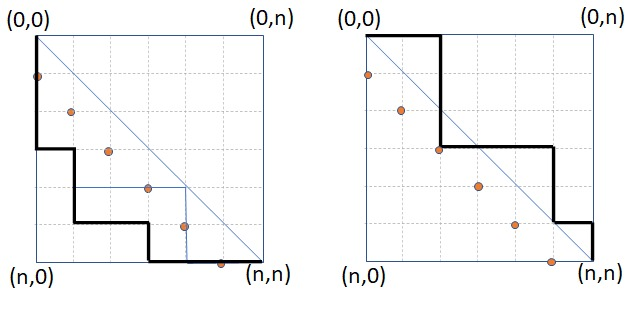
\includegraphics[width=0.7\linewidth]{images/diagonal-crossing.jpeg}
    \caption{Diagonal crossing paths. Note that path in (a) is crossing the diagonal at $(0,0)$}
    \label{fig:diagonal-crossing-path}
\end{figure}

\begin{figure}[h!]
    \centering
    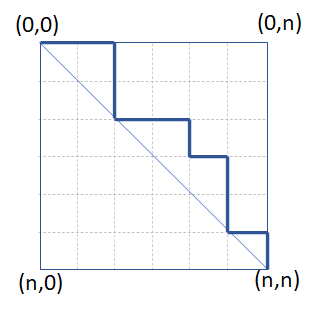
\includegraphics[width=0.4\linewidth]{images/diagonal-avoiding-path.png}
    \caption{A diagonal avoiding path. Observe that it can still touch the diagonal}
    \label{fig:diagonal-avoiding-path}
\end{figure}

Before computing this number, an obvious question is what is the connection between such restricted paths and Catalan number. It turns out that the set of diagonal avoiding paths from $(0,0)$ to $(n,n)$ is in bijection with the set of balanced paranthesized strings of length $2n$. Hence, to count the number of balanced paranthesized strings of length $2n$, which is also the Catalan number, we only need to count the diagonal avoiding paths from $(0,0)$ to $(n,n)$. Let us first establish the bijection between the two.

\subsection{Bijection from Diagonal avoiding paths to Balanced parenthesisation problem}
Intuitively, the bijection can be defined as follows: for any given balanced parenthesized string $w = w_1w_2\ldots w_{2n}$, the corresponding path from $(0,0)$ to $(n,n)$ is obtained by starting from position $(0,0)$, and scanning the string from left to right. Take  right move whenever $`('$ is encountered and a down move for $`)'$. Formally we define the bijection as follows:
\medskip{}

\noindent\underline{Defining the bijection:} Let $P$ be the set of diagonal avoiding paths from $(0,0)$ to $(n,n)$  and $B$ be the set of balanced paranthesized  strings of length $2n$ over the alphabets $\{(,)\}$. Define the bijection $\phi:B\rightarrow P$ as follows:\\
For $w=w_1 w_2 \ldots w_{2n}\in B$, $\phi(w) = (u_0,v_0), (u_1,v_1), \ldots, (u_i, v_i), \ldots, (u_{2n}, v_{2n})$, where 
\begin{enumerate}
    \item $(u_0,v_0)=(0,0)$ 
    \item $\forall i\in\{1,2,\ldots, 2n\}$\\
    \[
    (u_i, v_i) = 
    \begin{cases}  
    (u_{i-1}+1, v_{i-1})& ~~~~\text{if }w_i=)\\
    (u_{i-1}, v_{i-1}+1)&~~~~\text{if }w_i=(
    \end{cases}
    \]
    % $(u_i, v_i) = (u_{i-1}+1, v_{i-1})~~~~\text{if }w_i='('$\\
    % $(u_i, v_i) = (u_{i-1}, v_{i-1}+1)~~~~\text{if }w_i=')'$
\end{enumerate}
\underline{Proof of bijection}
\begin{description}
\item \textit{Well-defined:} From the above description, given any string $w$, $\phi(w)$ is uniquely defined. Further, for any string $w\in B$, since the number of $'('$ is same as  the number of $')' = n$, the corresponding path has $n$ right and $n$ down moves and hence it ends at $(n,n)$. Also, since the number of left brackets is greater than or equal to the number of right brackets in any prefix of $w$, for all $i\in[2n]$, $v_i\ge u_i$. This shows that $\forall w\in B, \phi(w)\in P$. Hence,  $\phi$ is well-defined.
\item \textit{Injective:} Let $w, w'$ be two different strings in set $B$. Then $\exists~$ an index $i\in[2n]$ where $w_i\ne w'_i$. Hence $\phi(w)$ and $\phi(w')$ also differ at the $i$th step, where one of the paths takes one step right while the other takes one step down. 
\item \textit{Surjective:} 
Given any path $((0,0), (u_1, v_1), \ldots, (u_{2n}, v_{2n}))$ the corresponding string $w\in B$ is defined as follows:\\
$\forall i\in[2n]$
\[
w_i = 
\begin{cases}
`(`& ~~~~~\text{if } (u_i, v_i) = (u_{i-1}, v_{i-1}+1)\\
`)`& ~~~~~\text{if } (u_i,v_i) = (u_{i-1}+1, v_{i-1})
\end{cases}
\]
We can verify that the string $w$ indeed is in set $B$, because firstly, for any path in $P$, $\forall i, v_i\ge u_i$ and hence by definition, number of left brackets $`(`$ in $w$ is greater than or equal to number of right brackets, $`(`$ in any prefix of $w$. Secondly, for any path to reach from $(0,0)$ to $(n,n)$ it must have $n$ right moves (increase in 2nd coordinate) and $n$ down moves (increase in 1st coordinate) and hence $w$ must have $n$ left brackets and $n$ right brackets.
\end{description}


% Properties:
% %$\phi(w_1)=u_1$ and $\phi(w_2)=u_2$ will be same till $(i-1)$th step, i.e. $(u_{1,(i-1)}, v_{1,(i-1)}=(u_{2,(i-1)}, v_{2,(i-1)}$ for $j=0$ to $i-1$.

\subsection{Counting the number of diagonal avoiding paths} 
Having established the bijection between Catalan number and diagonal avoiding paths, we get  
\begin{equation}
\label{eq:catalan-expr-1}
    C_n = \# \text{ of diagonal avoiding paths from } (0,0) to (n,n) 
\end{equation}
So, our next task is to count the number of diagonal avoiding paths from $(0,0)$ to $(n,n)$. 
To count this, we take following approach. Let us call the diagonal avoiding paths as \textit{good} paths and diagonal crossing paths as \textit{bad} paths. Then,
\begin{equation}
\label{eq:no-of-good-paths}
\Large
    \substack{\text{\# of diagonal avoiding paths }\\ \text{from } (0,0) \text{ to } (n,n)}  = \substack{\text{\# of paths }\\ \text{from } (0,0) \text{ to } (n,n)} - \substack{\text{\# of diagonal crossing paths }\\ \text{from } (0,0) \text{ to } (n,n)}
\end{equation}  

So, now our revised goal is to count the number of diagonal crossing paths from $(0,0)$ to $(n,n)$. How do we do that? Here again bijection plays an important role. The idea is to translate diagonal crossing paths into  different kind of paths which are easy to count. 

Let us define the following path translation:  Let $\pi=(0,0), (u_1,v_1), \ldots, (u_{2n}, v_{2n})$ be  a diagonal crossing path. Then there must exist $i$ such that $u_i = v_i+1$. There can be many such indices as the path can cross the diagonal multiple times. Choose $i$ to be the least such index. Let $u_i = \ell$, then the first co-ordinate after crossing the diagonal is $(\ell, \ell-1)$. Let us call this point $P$ (refer fig. \ref{fig:reflecting-path}(a)). Then to find the translated path we reflect the part of the path $\pi$ after point $P$ w.r.t. the main diagonal. 

\begin{figure}[h!]
    \centering
    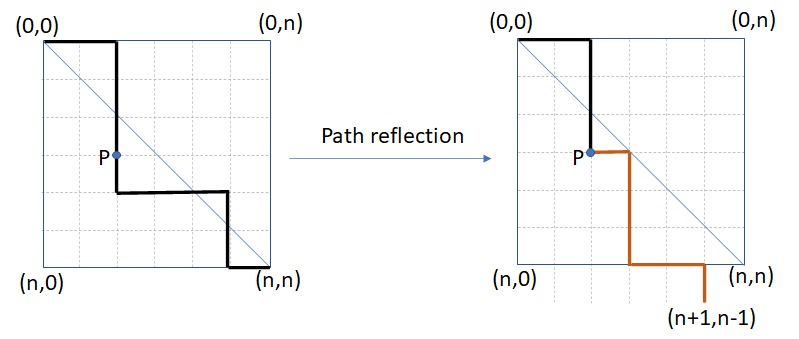
\includegraphics[width=0.7\linewidth]{images/reflecting-path.jpeg}
    \caption{Point P in a diagonal crossing path and the reflected path after P}
    \label{fig:reflecting-path}
\end{figure}

More precisely, we can divide the diagonal crossing path into two stretch $S_1, S_2$, where $S_1$ is the part of the path between $(0,0)$ to $P$ and $S_2$ is the part of the path between $P$  to $(n,n)$. 
Then to translate $\pi$ into a new path, replace $S_2$ with $S_2'$  to get a new path $\pi' = S_1S_2'$. The replacement $S_2'$ is defined as follows:
\begin{itemize}
    \item[-] replace downward edges with right edges and 
    \item[-] replace right edges with downward edges.
\end{itemize} Refer fig. \ref{fig:reflecting-path}(b)
We can observe that the new path $\pi'$ described in this way is always between $(0,0)$ to $(n+1, n-1)$. The argument for this goes as follows:

Originally (in $S_2$), $(\ell, \ell-1)$ goes to $(n,n)$ which means it takes $(n-\ell)$ downward moves and $(n-\ell+1)$ right moves. Since, we are swapping the right and downward moves to get $S_2'$ from $S_2$, there are $(n-\ell+1)$ downward moves and $(n-\ell)$ right moves from point $P=(\ell, \ell-1)$ in $S_2'$. Thus, $S_2'$ goes from $(\ell, \ell-1)$ to $(\ell+n-\ell+1, \ell-1+n-\ell) = (n+1, n-1)$ and hence, $\pi' = S_1S_2'$ is a path from $(0,0)$ to $(n+1, n-1)$. 

Thus we have established that any diagonal crossing path from $(0,0)$ to $(n,n)$ maps to a path from $(0,0)$ to $(n+1,n-1)$ after applying the transformation described above. The converse is also true, i.e., given any path from $(0,0)$ to $(n+1, n-1)$, we can translate it back to a diagonal crossing path from $(0,0)$ to $(n,n)$ by using the same reflection technique.  Thus, we get a bijection between the set of diagonal crossing paths from $(0,0)$ to $(n,n)$ to the set of paths from $(0,0)$ to $(n+1,n-1)$. We formally define the translation and prove that it is indeed a bijection.
\begin{description}
\item \underline{Bijection:}
Let $A$ be the set of diagonal crossing paths from $(0,0)$ to $(n,n)$ and $B$ be the set of paths from $(0,0)$ to $(n+1,n-1)$. Then the mapping $\phi:A\rightarrow B$ is formally defined as follows: 
\\
Let $\pi=(0,0), (u_1,v_1), \ldots, (u_{2n}, v_{2n})$ and $(u_i, v_i)$ be the first point when $\pi$ crosses the diagonal. Then $\phi(\pi) = \pi'=(0,0), (u'_1,v'_1), \ldots, (u'_{2n}, v'_{2n})$ is given by:
\begin{enumerate}
    \item $\forall 1\le j\le i, (u'_j, v'_j) = (u_j, v_j)$
    \item $\forall i+1\le j\le 2n$, 
    \[
    (u'_j, v'_j) = 
    \begin{cases}
    (u'_{j-1}+1, v'_{j-1})& ~~~~~\text{if } (u_j, v_j) = (u_{j-1}, v'_{j-1}+1)\\
    (u'_{j-1}, v'_{j-1}+1)& ~~~~~\text{if } (u_j, v_j) = (u_{j-1}+1, v'_{j-1})
    \end{cases}
    \]
\end{enumerate}
% We can verify that $\phi:A\rightarrow B$ satisfies all the properties of a bijection as follows:
\item \textit{Well-defined:} We already observed that any path $\pi\in A$ from $(0,0)$ to $(n,n)$ maps to a path $(0,0)$ to $(n+1,n-1)$. Hence $\phi$ is well defined.
\item \textit{Injection:} Consider two different diagonal crossing paths $\pi_1$ and $\pi_2$. Let $\pi_1 = S_{1,1}S_{1,2}$ and $\pi_2 = S_{2,1}S_{2,2}$, where the two components $S_{i,1}$ and $S_{i,2}$ for $i\in\{1,2\}$ are as defined before. Then following two cases are possible:
\begin{itemize}
    \item Case1: $S_{11}\ne S_{21}$. Then $\pi_1'\ne \pi_2'$, because the first component is copied as it is in the translation, i.e. $\pi_1' = S_{1,1}S_{1,2}'$ and $\pi_2' = S_{2,1}S_{2,2}'$.
    \item Case2: $S_{11}= S_{21}$, but $S_{12}\ne S_{22}$. In this case $S_{12}'\ne S_{22}'$ because of the way it is defined, i.e. for every right move there is a downwards move and vice-versa. Hence, $\pi_i'\ne \pi_2'$.
\end{itemize}
\item \textit{Surjective:} Given any path $\pi'$ from  $(0,0)$ to $(n+1,n-1)$, we can construct the corresponding path $\pi$ from $(0,0)$ to $(n,n)$, such that $\phi(\pi) = \pi'$, as follows.\\
Let $\pi'=(0,0), (u'_1,v'_1), \ldots, (u'_{2n}, v'_{2n})$. Since $\pi'$ goes to $(n+1, n-1)$ which is below the diagonal there must exist $i$ such that $(u'_i,v'_i)$ is below the diagonal. Again, there can be many such indices. Take $i$ to be the first such index. Same as before, let $\pi' = S_1'S_2'$, where $S_1'$ is the path from $(0,0)$ to $(u_i', v_i')$ and  $S_1'$ is the path from $(u_i',v_i')$ to $(u_{2n}', v_{2n}')$. Then $\pi = S_1'S_2$ where $S_2$ is obtained from $S_2'$ by swapping the right and downwards moves. Mathematically, let $\pi=(0,0), (u_1,v_1), \ldots, (u_{2n}, v_{2n})$. Then
\begin{enumerate}
    \item $\forall j\le i$, $(u_j, v_j) = (u_j', v_j')$
    \item $\forall~i+1\le j\le 2n$
    \[
    (u_j, v_j) =
    \begin{cases}
    (u_{j-1}+1, v_{j-1}) & ~~~~~\text{if } (u_j', v_j') = (u_{j-1}', v_{j-1}'+1)\\
    (u_{j-1}, v_{j-1}+1) & ~~~~~\text{if } (u_j', v_j') = (u_{j-1}'+1, v_{j-1}')
    \end{cases}
    \]
\end{enumerate}
Again by the same argument as before it can be verified that $\pi$ is a diagonal crossing path from $(0,0)$ to $(n,n)$. We write it here for completeness. Let $(\ell, \ell-1)$ be the first point when $\pi'$ crosses the diagonal. Then since the path from $(0,0)$ to $(\ell, \ell-1)$ remains as it is in $\pi$, it is a diagonal crossing path. Further since $\pi'$ is path from $(0,0)$ to $(n+1, n-1)$, it takes $n+1-\ell$ downward steps and $n-\ell$ right steps from $(\ell, \ell-1)$. Hence, $\pi$ takes $n+1-\ell$ right and $n-\ell$ downward steps from $(\ell, \ell-1)$. Thus, $\pi$ ends at $(\ell+n-\ell, \ell-1+n+1-\ell) = (n,n)$. 
\end{description}

Thus, we have established a bijection between the set of diagonal crossing paths from $(0,0)$ to $(n,n)$ and the set of  paths from $(0,0)$ to $(n+1,n-1)$. Hence, 
\begin{eqnarray*}
    \# \text{of diagonal crossing paths from } (0,0) \text{ to } (n,n) &=& \# \text{of paths from } (0,0) \text{ to } (n+1,n-1)\\
    &= &{2n\choose n+1}
\end{eqnarray*}
Hence, from~\eqref{eq:catalan-expr-1},\eqref{eq:no-of-good-paths},
\begin{align*} %\label{eq:no-of-good-paths-2}
C_n &= \# \text{of diagonal avoiding paths from} (0,0) \text{ to } (n,n)\\
%\Large
 %   \substack{\text{\# of diagonal avoiding paths }\\ \text{from } (0,0) \text{ to } (n,n)} 
     &= \Large \substack{\text{\# of paths }\\ \text{from } (0,0) \text{ to } (n,n)} - \Large\substack{\text{\# of diagonal crossing paths }\\ \text{from } (0,0) \text{ to } (n,n)}\\
    &= {2n\choose n} - {2n\choose n+1}\\
    & = {2n\choose n} - \frac{n}{n+1}{2n\choose n}\\
    &=\frac{1}{n+1}{2n\choose n}
\end{align*}  

Here, in the second last line, we have used the identity: $${2n\choose n+1} = \frac{n}{n+1}{2n\choose n}.$$









% Let us define the following path translation: Let $p=(0,0), (u_1,v_1), \ldots, (u_{2n}, v_{2n})$ be  a diagonal crossing path which goes below the diagonal at point $(u_i, v_i)$ for for the first time. Then, translate the path $p$ to a new path $p' = (u'_0, v'_0), (u'_1,v'_1), \ldots, (u'_{2n}, v'_{2n})$ by \textit{reflexing} $p$ between  $(u_i, v_i)$ and $(u_{2n}, v_{2n})$ in the sense that whenever $p$ goes right, $p'$ goes down, and whenever $p$ goes down, $p'$ moves right. Mathematically,
% \begin{enumerate}
%     \item $\forall 1\le j\le i, (u'_j, v'_j) = (u_j, v_j)$
%     \item $\forall i+1\le j\le 2n$, 
%     \[
%     (u'_j, v'_j) = 
%     \begin{cases}
%     (u'_{j-1}+1, v'_{j-1})& ~~~~~\text{if } (u_j, v_j) = (u_{j-1}, v'_{j-1}+1)\\
%     (u'_{j-1}, v'_{j-1}+1)& ~~~~~\text{if } (u_j, v_j) = (u_{j-1}+1, v'_{j-1})
%     \end{cases}
%     \]
% \end{enumerate}
% In the example, we can see that the translated path ends up at $(n+1, n-1)$. In general, we can prove the following: The above defined translation of any diagonal crossing path $p$ from $(0,0)$ to $(n,n)$ always ends at $(n+1, n-1)$.
% \begin{proof}
% Let $p$ croses the diagonal for the first time at $(u_i, v_i)$. Then 
% $$u_i = v_i+1.$$ 
% From $(u_i, v_i)$, $p$ moves $(n-u_i)$ steps down and $(n-v_i)$ steps in the right to reach $(n,n)$. Hence, the translated path $p'$ takes $(n-u_i)$ steps right and $(n-v_i)$ steps down from $(u_i, v_i)$ and ends at $$ (u_i+n-v_i, v_i+n-u_i) = (n+(u_i-v_i), n+(v_i-u_i)) = (n+1, n-1)$$. 
% \end{proof}

% Conversely, any path $p'$ from $(0,0)$ to $(n+1, n-1)$ can be mapped to a diagonal crossing path from $(0,0)$ to $(n,n)$. Intuitively, this can be done by again reflecting it  from the point $(u_i, v_i)$, where it crosses the diagonal for the first time. Note that such a point always exist because to reach the point $(n+1, n-1)$ $p'$ must cross the diagonal because $(n+1, n-1)$ is below the diagonal. Using the same argument as above, it can be shown that this translates $p'$ into a diagonal crossing path from $(0,0)$ to $(n,n)$.

% Thus, we get a bijection between the set of diagonal crossing paths from $(0,0)$ to $(n,n)$ and the set of paths from $(0,0)$ to $(n+1,n-1)$ defined formally as follows:\\

% Definition: Let $A$ be the set of diagonal crossing paths from $(0,0)$ to $(n,n)$ and $B$ be the set of paths from $(0,0)$ to $(n+1,n-1)$. Then a bijection $\phi:A\rightarrow B$ is defined as follows:

% For any path $p = (u_0, v_0), (u_1, v_1), \ldots, (u_{2n}, v_{2n})\in A$, let $(u_i, v_i)$ be the point where the path crosses the diagonal for the first time. That is, 
% \begin{enumerate}
%     \item $\forall j<i, v_j\ge u_j$, and
%     \item $u_i=v_i+1$
% \end{enumerate}
% Then $\phi(p)=p' = (u'_0, v'_0), (u'_1, v'_1), \ldots, (u'_{2n}, v'_{2n})$, where
% \begin{enumerate}
%     \item 
% \end{enumerate}
\begin{ex}
\item Try to establish a bijection between the set of different possible polygon triangulation in a polygon of $n+2$ nodes and the set of binary trees with $n$ internal nodes.

\textit{Hint: associate each internal node with a triangle in a triangulation. Then, each internal node will have degree three, which is the case for full binary tree, except for the leaves. Leaves will correspond to those triangles whose one of the edge is the boundary of the polygon.}
\end{ex}

 

\Lecture{Jayalal Sarma}{Sept 19, 2020}{07}{From Bijections to PIE}{Anshu Yadav}{$\alpha$}{JS}

\section{Introduction}
In this lecture, we will continue with the use of bijections and use it in formally proving the two identities that we discussed in class and then see their relationship to the Principal of Inclusion and Exclusion. 

\section{The Identities}
Recall that we proved following two identities in one of the discussion sessions
\begin{align}
     \sum_{k=0}^n (-1)^k{n\choose k} &= 0 \label{REV1}\\ 
     \sum_{k=0}^m (-1)^k{n\choose k} &= (-1)^m{n-1\choose m} \label{REV2}
\end{align}
In this section, we will see the proofs for the above equations is detail
\subsection{Proof for Eqn. \eqref{REV1}} \label{subsec:identity-even-odd-1}
$$\sum_{k=0}^n (-1)^k{n\choose k} = 0$$
\begin{proof}
    The LHS counts the number of even sized subsets of $[n]$ with positive sign and odd size subsets with negative sign. Then we proved the result using bijection between even sized and odd sized subsets of $[n]$. Hence, we get 0 on RHS. Let us formally define the bijection here.
    
    Let $E$ be the set of all even sized subsets of $[n]$ and $O$ be the set of all odd sized subsets of $[n]$. Then the bijection  $\phi_i:E\rightarrow O$ is defined with respect to an element $i\in[n]$ as follows.
    
    Let $X\subseteq [n]$, such that $|X|$ is even. Then 
    \[
        \phi_i(X) = 
        \begin{cases}
            X\setminus \{i\} & ~~~~~\text{ if } i\in X\\
            X\cup\{i\} & ~~~~~\text{ if } i\not\in X
        \end{cases}
    \]
    \underline{Proof of bijection:}
    \begin{description}
        \item \textit{Well-defined:} Given any even sized subset $X$, there are two possibilities: (i) $i\in X$, (ii) $i\not\in X$. In first case, $i$ is removed from $X$, hence its size reduces by one and becomes odd. In the second case, $i$ is added, hence the size of the subset increases by one and becomes odd. Hence, $\phi$ is well defined.
        \item \textit{Injective:} Let $X$ and $X'$ be two distinct subsets of $[n]$. Then $\exists j\in[n]$ such that $j$ is present in exactly one of the two subsets. Wlog, let $j\in X$ and $j\not\in X'$. Now, if $j\neq i$, then $j\in \phi(X)$ and $j\not\in \phi(X')$ and hence $\phi(X)\neq \phi(X')$. On the other hand, if $j=i$, then $j\not\in \phi(X)$ and $j\in \phi(X')$. Hence, $\phi(X)\neq \phi(X')$.  
        \item \textit{Surjective:} Let $Y\in O$ be an odd sized subset of $[n]$. From $Y$, we can recover $X$ such that $\phi(X) = Y$ by the same operation as in $\phi$. That is, 
        \[
        X= \begin{cases}
            Y\setminus \{i\} & ~~~~~\text{ if } i\in Y\\
            Y\cup\{i\} & ~~~~~\text{ if } i\not\in Y
        \end{cases}
        \]
        It can easily be verified that in both the cases, $X$ is an even sized subset of $[n]$.
    \end{description}
    This completes the proof.
\end{proof}
%
%
\subsection{Proof for Eqn. \eqref{REV2}} \label{subsec:identity-even-odd-2}
$$\sum_{k=0}^m (-1)^k{n\choose k} = {n-1\choose m}$$
\begin{proof}
Now we look at the second identity which is even more interesting. To prove this identity we use \emph{almost bijection} where the bijection is between a set and subset of another set.

In words, the identity to prove, can be described as
$$\Large\substack{\# \textrm{ of even sized subsets of  $[n]$}\\  \textrm{of size atmost $m$}} - \substack{\# \textrm{ of odd sized subsets of $[n]$} \\ \textrm{of size atmost $m$}} = (-1)^m{n-1\choose m}.$$ Clearly, there cannot be a bijection between the two sets (even sized subsets and odd sized subsets) in this case, since their difference is non-zero. This is where we use almost bijection.

We use following case analysis. 
\begin{description}
\item \underline{\textbf{Case1:} $m$ is even:} Then the identity to prove is:
\begin{equation} \label{eq:even-odd}
    \sum_{k=0}^m (-1)^k{n\choose k} = {n-1\choose m}
\end{equation}
This can be interpreted as 
\begin{equation} \label{eq:even-odd-1}
    \sum_{\substack{k=0,\\k\text{ is even}}}^m {n\choose k} -  \sum_{\substack{k=1,\\k\text{ is odd}}}^{m-1} {n\choose k} = {n-1\choose m}
\end{equation}
Let $E$ be the set of all the even sized subsets of $[n]$ of size at most $m$ and $O$ be the set of odd sized subsets of $[n]$ having size at most $m-1$. Then, Eqn.~\eqref{eq:even-odd-1} can intuitively interpreted as follows: there is a subset $E'\subseteq E$, such that $E'$ is in bijection with $O$ and $|E\setminus E'| = {n-1\choose m}$. Thus, we have three tasks at hand
\begin{itemize}
    \item identify the set $E'$, and
    \item define and prove the bijection between $E'$ and $O$.
    \item prove that $|E\setminus E'| = {n-1\choose m}$
\end{itemize}
\underline{Defining the set $E'$:} Set $E'$ is the union of two sets: 
$$E' = \{X\subseteq [n]: |X| \textrm{ is even and } |X|\le m-2\}\cup\{X\subseteq [n]: i\in X \textrm{ and } |X| = m\}$$
\underline{Defining the bijection:} The bijection $\phi:E'\rightarrow B$ is defined in the same way as we defined it for first identity. That is, for $X\in E'$,
\[
\phi(X) = 
\begin{cases}
X\setminus \{i\} & ~~~~~\text{ if } i\in X\\
X\cup\{i\} & ~~~~~\text{ if } i\not\in X
\end{cases}
\]
\underline{Proof of bijection}
\begin{description}
\item \textit{Well-defined:} Let $X\in E'$, then (i) if $|X|\le m-2$, then $|\phi(X)|$ is odd and $|\phi(X)|\le m-1$, (ii) if $|X| = m$, then $i\in X$, hence $\phi(X) = X\setminus \{i\}$. This implies $|\phi(X)| = m-1$. Thus, in both the cases $\phi(X)\in O$.
\item \textit{Injective:} Since, the function is same as in the previous case, the same argument for injectivity works.
\item \textit{Surjective:} Let $Y\in O$ be an odd sized subset of $[n]$. From $Y$, we can recover $X\in E'$ such that $\phi(X) = Y$ by the same operation as in $\phi$. That is, 
 \[
 X= 
 \begin{cases}
Y\setminus \{i\} & ~~~~~\text{ if } i\in Y\\
Y\cup\{i\} & ~~~~~\text{ if } i\not\in Y
 \end{cases}
 \]
 It can easily be verified that in both the cases, $|X|$ is even. 
 In first case, since $|Y|\le m-1, |X|\le m-2$, hence $X\in E'$. In second case, since $i\not\in Y$ and $|Y|\le m-1$, $|X|\le m$ and $i\in X$. Hence $X\in E'$, by definition.
\end{description}
This proves the bijection between $E'$ and $O$. 

\underline{Proof for: $|E\setminus E'| = {n-1\choose m}$}

From the above definitions, $E\setminus E' = \{X\subseteq [n]: |X| = m, i\not\in X\}$. This can be interpreted as $E\setminus E' = \{X\subseteq [n]\setminus \{i\}: |X| = m\}$. Hence, $|E\setminus E'| = {n-1\choose m}$.

\item \underline{\textbf{Case2:} $m$ is odd:} In this case the identity to prove is:
\begin{equation}
\label{eq:even-odd-3}
    \sum_{k=0}^m (-1)^k{n\choose k} = - {n-1\choose m}
\end{equation}
This can be interpreted as 
\begin{equation}
\label{eq:even-odd-2}
    \sum_{\substack{k=0,\\k\text{ is even}}}^{m-1} {n\choose k} -  \sum_{\substack{k=1,\\k\text{ is odd}}}^{m} {n\choose k} = -{n-1\choose m}
\end{equation}
Equivalently,
\begin{equation}
\label{eq:odd-even-1}
    \sum_{\substack{k=1,\\k\text{ is odd}}}^{m} {n\choose k} - \sum_{\substack{k=0,\\k\text{ is even}}}^{m-1} {n\choose k}  = {n-1\choose m}
\end{equation}
This time the set of odd sized subsets of $[n]$ of size at most $m$ is bigger than the even sized subsets of $[n]$ of size at most $m$.
The proof is same as that for the case of even $m$. 
Let $E$ be the set of all the even sized subsets of $[n]$ of size at most $m-1$ (since $m$ is odd) and $O$ be the set of odd sized subsets of $[n]$ having size at most $m$. Then~\eqref{eq:odd-even-1} can be interpreted as follows: there is a subset $O'\subseteq O$, such that $E$ is in bijection with $O'$ and $|O\setminus O'| = {n-1\choose m}$.
  
Thus, we have two task at hand
\begin{itemize}
    \item identify the set $O'$, and
    \item define and prove the bijection between $E$ and $O'$.
    \item prove that $|O\setminus O'| = {n-1\choose m}$
\end{itemize}
\underline{Defining the set $O'$:} Set $O'$ to be the union of two sets: 
$$O' = \{Y\subseteq [n]: |Y| \text{ is odd and } |Y|\le m-2\}\cup\{Y\subseteq [n]: i\in Y \text{ and } |Y| = m\}$$
\underline{Defining the bijection:} The bijection $\phi:E\rightarrow O'$ is defined in the same way as we defined it for first identity. That is, for $X\in E$,
\[
\phi(X) = 
\begin{cases}
X\setminus \{i\} & ~~~~~\text{ if } i\in X\\
X\cup\{i\} & ~~~~~\text{ if } i\not\in X
\end{cases}
\]
\underline{Proof of bijection}
\begin{description}
\item \textit{Well-defined:} Let $X\in E$, then $\phi(X)$ is of odd size because either an element is added or removed from $X$, which is of even size. Now, (i) if $i\in X$, then $\phi(X) = X\setminus\{i\}$. Hence, $|\phi(X)|\le m-2$ (because $|X|\le m-1$) which implies $\phi(X)\in O'$ (ii) if $i\not\in X$, then, $\phi(X) = X\cup \{i\}$. This implies $|\phi(X)| \le m$. But since, $i\in \phi(X)$, $\phi(X)\in O'$. This proves that $\phi$ is well- defined.
\item \textit{Injective:} Since, the function is same as in sub section~\ref{subsec:identity-even-odd-1}, the same argument for injectivity works.
\item \textit{Surjective:} Let $Y\in O'$ be an odd sized subset of $[n]$. From $Y$, we can recover $X\in E$ such that $\phi(X) = Y$ by the same operation as in $\phi$. That is, 
 \[
 X= 
 \begin{cases}
Y\setminus \{i\} & ~~~~~\text{ if } i\in Y\\
Y\cup\{i\} & ~~~~~\text{ if } i\not\in Y
 \end{cases}
 \]
 It can easily be verified that in both the cases, $|X|$ is even. 
 In first case, $|Y|\le m$ and hence $|X|\le m-1$. So, $X\in E$. In second case, since $i\not\in Y$, $|Y|\le m-2$ (by definition) and hence $|X|\le m-1$. Hence $X\in E$.
\end{description}
This proves the bijection between $E$ and $O'$. 

\underline{Proof for: $|O\setminus O'| = {n-1\choose m}$}\\
From the above definitions, $O\setminus O' = \{Y\subseteq [n]: |Y| = m, i\not\in Y\}$. This can be interpreted as $O\setminus O' = \{Y\subseteq [n]\setminus \{i\}: |Y| = m\}$. Hence, $|O\setminus O'| = {n-1\choose m}$.
\end{description}
This completes the proof
\end{proof}
This proves both the identities.
%%%%%%%%%%%%%%%%%%%%%%%%%%%%%%%%%%%%%%%%%%%%%%%%%%%%%%%%%%%%%%%%%%%%%%%%%%%%%
\section{Principle of Inclusion and Exclusion}
Suppose we are given $n$ sets $A_1, A_2, \ldots, A_n\subseteq G$, where $G$ is some ground set. We are interested in finding the size of $A= A_1\cup A_2\cup\ldots\cup A_n$. This is very abstract scenario and we will see specific examples later, but here we are going to see classic use of the above identities in deriving this number.

So, we are interested in finding $|A| = |A_1\cup A_2\cup\ldots\cup A_n|$. 

So, here is a thought process - 
Clearly, we can add the size of individual sets as 
$|A| = |A_1|+|A_2|+\ldots +|A_n|$, but this will over-count if there are some elements present in more than one sets. So, for that we need to subtract the double counting. For e.g. if $x\in A_1$ and $x\in A_2$, then it gets counted twice and to compensate for that we need to subtract $|A|=|A_1\cap A_2|$ and we might attempt $|A| = |A_1|+|A_2|+\ldots +|A_n| - \sum_{1\le i < j\le n}|A_i\cap A_j|$. But then, if $x$ is present in $A_1, A_2$ and $A_3$, the it is under-counted (added thrice and subtracted thrice). So, again we need to compensate for that by adding $\sum_{1\le i \le j\le k\le n}|A_i\cap A_j\cap A_k|$ in the above expression and this sequence goes on for any element being present in $k\le n$ sets and finally we get the expression for $|A|$  as follows
\begin{equation} \label{eq:pie-1}
    |A| = |A_1|+\cdots+|A_n|-\sum_{1\le i< j\le n}|A_i\cap A_j| +\sum_{1\le i<j<k}|A_i\cap A_j\cap A_k| -\cdots + (-1)^{n+1}|A_1\cap A_2\cap\cdots\cap A_n|
\end{equation}
For $n=2$, the above expression gives
$$|A| = |A_1|+|A_2|-|A_1\cap A_2|$$
which we all must have seen before and can easily prove using Venn diagram. 

In this section, we will formally prove the above expression for general $n$ using the two identities we proved in previous section.
\begin{proof}
Consider any $x\in A_1\cup A_2\cup\cdots\cup A_n$. Let $x$ appears in $k$ of the $A_i$'s. Then let us see how $x$ gets counted
\begin{itemize}
    \item[-] $|A_1|+|A_2|+\cdots +|A_n|$: counts $x$ $k$ times (added)
    \item[-] $\sum_{1\le i<j\le n}|A_i\cap A_j|$: counts $x$ ${k\choose 2}$ times (subtracted)
    \item[-] $\sum_{1\le i<j<k\le n}|A_i\cap A_j\cap A_k|$: counts $x$ ${k\choose 3}$ times (added) 
    \item[-] and so on $\ldots$
\end{itemize}
Notice that in terms involving intersection of more than $k$ sets, $x$ never appears.

Thus, 
\begin{eqnarray*} 
{\Large\substack{\# \text{of times $x$}\\ \text{gets counted}}} &=& k+{k\choose 2}-{k\choose 3}+\cdots +(-1)^{k+1}{k\choose k}\\
&=&-{k\choose 0}+{k\choose 1}+{k\choose 2}-{k\choose 3}+\cdots +(-1)^{k+1}{k\choose k}+{k\choose 0}\\
&=&-\sum_{i=0}^k(-1)^{i}{k\choose i}+{k\choose 0}\\
%&&\text{from~\eqref{eq:identity-1}, $\sum_{i=0}^k(-1)^k{k\choose i} = 0$}\\
&=&{k\choose 0} ~~~~~~~~~~~~~~~~~~~~~~~\text{from ~\eqref{REV1}}\\
&=& 1
\end{eqnarray*}
Thus, irrespective of the value of $k$, any element $x\in A_1\cup A_2\cup\cdots\cup A_n$ is counted exactly once. Hence, every $x\in A_1\cup A_2\cup\cdots\cup A_n$ is counted exactly once in RHS in~\eqref{eq:pie-1}.

This proves the PIE
\end{proof}
Now let us look at the application of second identity that we derived. This identity is used in deriving a version of PIE which appears very naturally in several context. Let us look at one such example.

PIE says that if we want to derive $|A_1\cup\A_2\cup\cdots\cup A_n|$, then the following expression does not give the correct count.
$$|A_1\cup\A_2\cup\cdots\cup A_n| = |A_1|+|\A_2|+\cdots+|A_n|$$ 
But we can ask, does this expression gives a lower or an upper bound? As we saw, this does over-counting, hence we can write
$$|A_1\cup\A_2\cup\cdots\cup A_n| \le |A_1|+|\A_2|+\cdots+|A_n|$$
Now, suppose we include the next component, i.e. $$|A_1|+|\A_2|+\cdots+|A_n|-\sum_{1\le i<j\le n}|A_i\cap A_j|$$
Again from PIE we know that this also does not give the correct count. But we ask the same question again - does it give any lower or upper bound. And as we saw that this term can do some over-subtraction and hence we can say that this expression gives the lower bound. That is, 
$$|A_1\cup\A_2\cup\cdots\cup A_n| \ge |A_1|+|\A_2|+\cdots+|A_n|-\sum_{1\le i<j\le n}|A_i\cap A_j|$$
Similarly, 
$$|A_1\cup\A_2\cup\cdots\cup A_n| \le |A_1|+|\A_2|+\cdots+|A_n|-\sum_{1\le i<j\le n}|A_i\cap A_j|+\sum_{1\le i<j<k\le n}|A_i\cap A_j\cap A_k|$$
and we continue like this. 

Let us now formally establish this observation. We use the same technique that we used in the proof of PIE. 

Let $x$ appears in $k$ of the sets in $A_1, A_2, \ldots, A_n$. Suppose we cut off the PIE after $m\le n$ sized intersections. Then 
\begin{eqnarray*} 
{\Large\substack{\# \text{of times $x$}\\ \text{gets counted}}} &=& {k\choose 1}-{k\choose 2}+\cdots+(-1)^{m+1}{k\choose m}\\
%&=&-{k\choose 0}+{k\choose 1}+{k\choose 2}-{k\choose 3}+\cdots +(-1)^{k+1}{k\choose k}+{k\choose 0}\\
&=&-\sum_{i=0}^m(-1)^{i}{k\choose i}+{k\choose 0}\\
%&&\text{from~\eqref{eq:identity-1}, $\sum_{i=0}^k(-1)^k{k\choose i} = 0$}\\
&=& 1+(-1)^{m+1}{k-1\choose m} ~~~~~~~~~~~~~~~~~~~~~~~\text{from ~\eqref{REV2}}
\end{eqnarray*}
Thus, $x$ is over counted or under counted depending on whether the second term on RHS is positive or negative. Let us analyze this for two cases.
\begin{description}
\item Case1: $k\le m$

Since, $x$ appears in only $k\le m$ sets and we are cutting down only after $m$, then this means that all possible intersections of this particular $x$ are added and subtracted and $x$ can not appear in any of the intersections of more than $k$ sets. Hence, $x$ is neither under counted nor over counted. In the expression, ${k-1\choose m} = 0$ Hence,
$$\# \text{of times $x$ is counted } = 1$$
\item Case2: $k>m$

In this case, $x$ can be under counted or over counted depending upon whether $m$ is even or odd.
If $m$ is odd then $x$ is over counted.

If $m$ is even then $x$ is under counted.
\end{description}
Notice that either all $x\in A_1\cup\A_2\cup\cdots\cup A_n$ are correctly counted or under counted or all $x$ are correctly counted or over counted based on the parity of $m$. Thus, whether a PIE cut down after $m$ intersections gives lower bound or upper bound depends only on the parity of $m$. This principle is also called the \emph{Bon Ferroni's inequality}. 
\begin{remark} 
    We used the equality in~\eqref{eq:even-odd} to prove PIE. We can actually do the other way round as well, i.e. we can use PIE to prove this equality too.
\end{remark}
This completes this lecture. In the next lecture we will look at some applications of PIE.

%\Lecture{Jayalal Sharma}{Sept 19, 2020}{08}{Live lecture discussion}{Anshu and Narasimha Sai }{$\alpha$}{JS}

\section{Discussions}

\paragraph{Bijection from Euler's problem to Binary Trees} As we have already established a bijection from set of balanced parenthesisations to set of full binary trees and established that number of full binary trees with $n$ internal nodes is the catlan number $C_n$, in this section, let's establish a bijection from the \emph{Euler's Problem} to set of full binary trees to establish that the solution to \emph{Euler's problem} is also catlan number $C_n$.

Lets recall \emph{Euler's problem} first. Consider a convex polygon with $n+2$ edges. Euler's problem is the number of ways of triangulating it (partition the polygon into triangles) by drawing non-crossing diagonals. (Refer fig. \ref{fig:Euler's-polygon}). We know that number of non-crossing diagonals in a polygon of $n+2$ edges is $n-1$ (proof follows from a simple induction) and from those $n-1$ non-crossing diagonals, we have our polygon partitioned into $n$ triangles. Let's associate each of the triangles with a vertex (green dots in the fig. \ref{fig:Euler's-polygon}). Observe that if two triangles share an edge, it must be one of the diagonals (no two triangles can share an edge because of non-crossing diagonals). Now, let's connect the vertices whose corresponding triangles share an edge. Any edge connecting two of these vertices crosses a diagonal. 
\begin{figure}[h!]
    \centering
    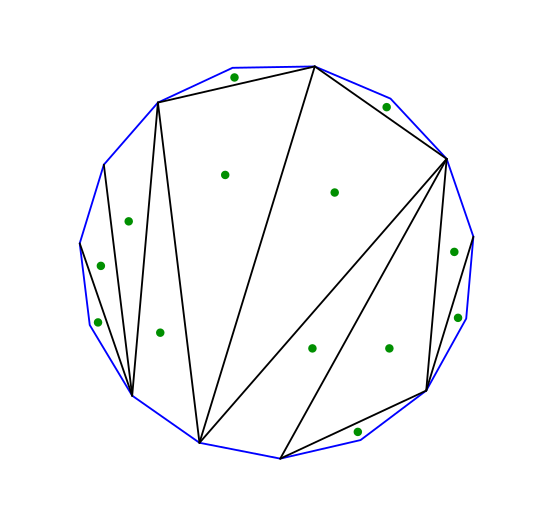
\includegraphics[width=0.4\linewidth]{images/polygon.png}
    \caption{Partitioning a polygon into triangles by non-crossing diagonals. Observe that green dots in each triangle associates the triangle with a vertex}
    \label{fig:Euler's-polygon}
\end{figure}
Now, consider a polygon edge $e$. For every polygon edge surrounding a vertex (other than $e$), add an open-edge originating from that vertex (see fig. \ref{fig:tree-in-polygon}). We arrive at the following claim.  
\begin{claim}
	If we remove the underlying triangles (which are formed with polygon edges and diagonals), from fig. \ref{fig:tree-in-polygon}, the 		resulting graph obtained (see fig. \ref{fig:tree}) is a full binary tree with the vertices as internal nodes.
\end{claim}
\begin{figure}[h!]
    \centering
    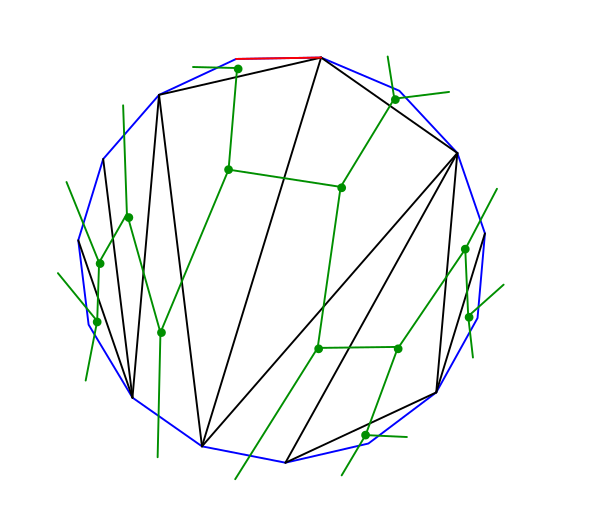
\includegraphics[width=0.4\linewidth]{images/polygon-tree.png}
    \caption{Polygon with vertices connected to form a tree}
    \label{fig:tree-in-polygon}
\end{figure}
\begin{figure}[h!]
    \centering
    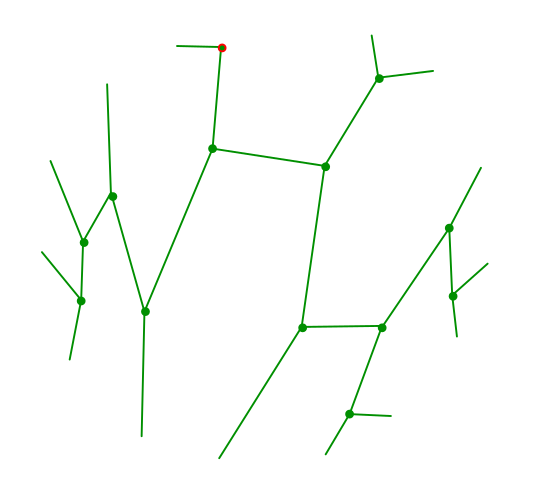
\includegraphics[width=0.4\linewidth]{images/tree.png}
    \caption{Tree formed by connecting vertices}
    \label{fig:tree}
\end{figure}
\begin{proof}
	We observe that degree of every vertex other than the vertex surrounded by edge $e$ is 2. This vertex will act as root to our full binary tree. All other vertices have degree 3 because each vertex is surrounded by a triangle and if a side is a diagonal, it will be connected to vertex which is surrounded by triangle that shares the diagonal and if the side is a polygon edge, then there will be an open edge corresponding to it originating from the vertex. Therefore the resulting graph formed is a full binary tree with our vertices as $n$ internal nodes and vertices corresponding to open edges are $n+1$ leaves (because there are $n+2$ edges and one edge is under consideration). This completes the description of bijection.
\end{proof}

We leave it as an exercise to the reader to prove that the mapping defined above is indeed a bijection.

\paragraph{Bijection from binary trees to full binary trees}
In this section we are interested in connection between binary and full binary trees. Recall that a full binary tree is one in which each node has either 0 or two children. On the other hand, when we say binary tree then it only means that each node can have at most two children. We want to find a bijection between set of binary trees with $n$ internal nodes and set of full binary trees with certain number of internal nodes. 

First of all lets try to see how to convert a given binary tree into a full binary tree so that we can reverse the process, i.e. recover the original (binary) tree back from the full binary tree without ambiguity. 

Here is the first attempt:

\noindent \underline{Attempt 1:} First natural approach can be to add a leaf node to all non-full (internal nodes having only one child) nodes, as shown in figure~\ref{fig:bt-fbt-attempt1}
\begin{figure}[h!]
    \centering
    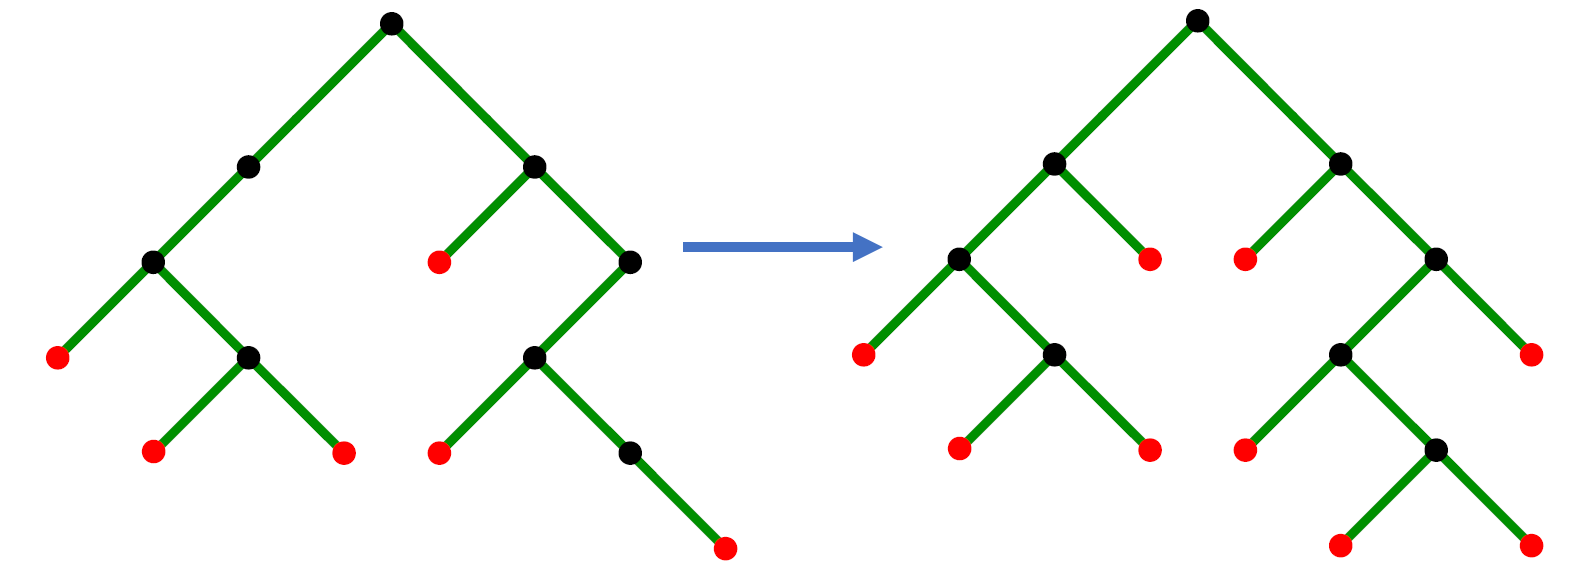
\includegraphics[width=0.7\linewidth]{images/binary-to-full-binary-1.png}
    \caption{Binary to full binary tree attempt1: adding a child node to each non full node}
    \label{fig:bt-fbt-attempt1}
\end{figure}

But notice that this transformation is not injective. For example, it can be observed that  both the trees in figure~\ref{fig:bt-fbt-attempt1-issue} map to same full binary tree.
\begin{figure}[h!]
    \centering
    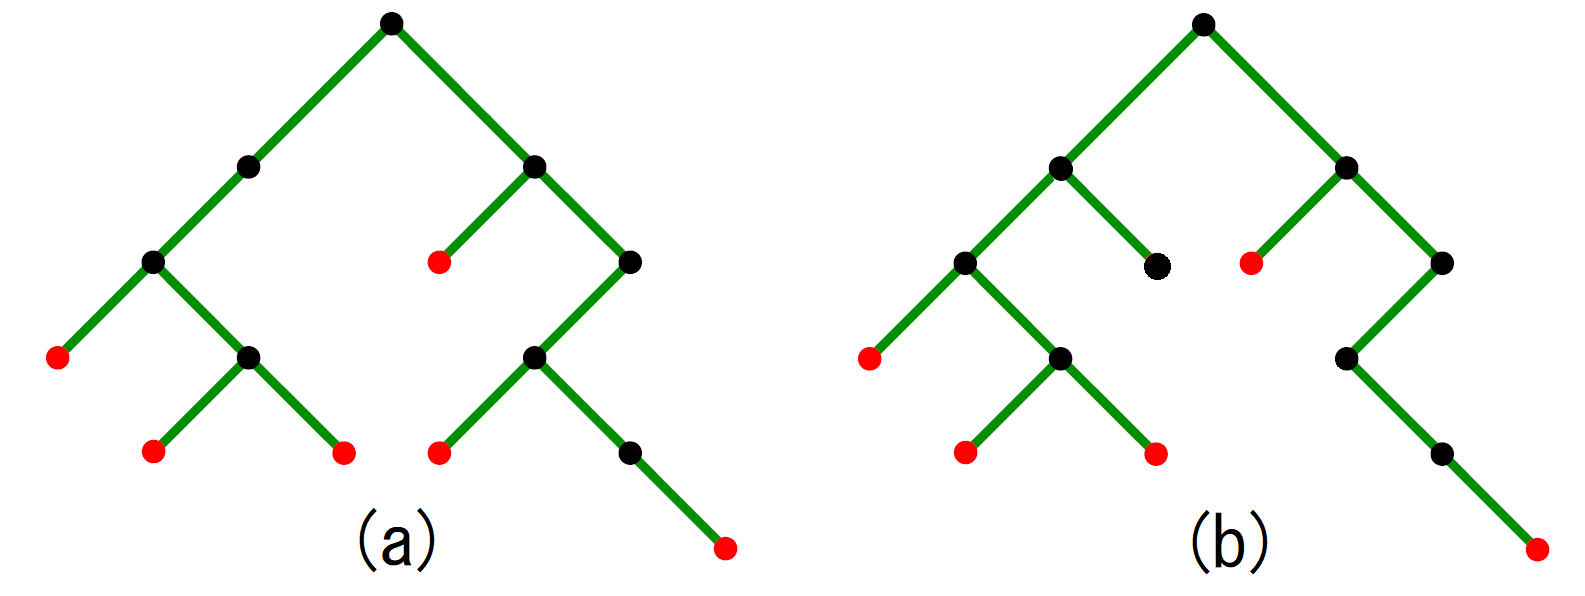
\includegraphics[width=0.7\linewidth]{images/binary-to-full-binary-2.png}
    \caption{Two different binary trees that map to same full binary tree}
    \label{fig:bt-fbt-attempt1-issue}
\end{figure}

\noindent\underline{Attempt 2(correct)}
Lets try a slightly different approach. Given a binary tree, do the following:
\begin{itemize}
    \item to each leaf node, add two children
    \item to each internal node having only one child, add another child
\end{itemize}
Figure~\ref{fig:binary-to-full-solution} shows the full binary tree constructed in this way for the same binary tree as in Figure~\ref{fig:bt-fbt-attempt1}.
\begin{figure}[h!]
    \centering
    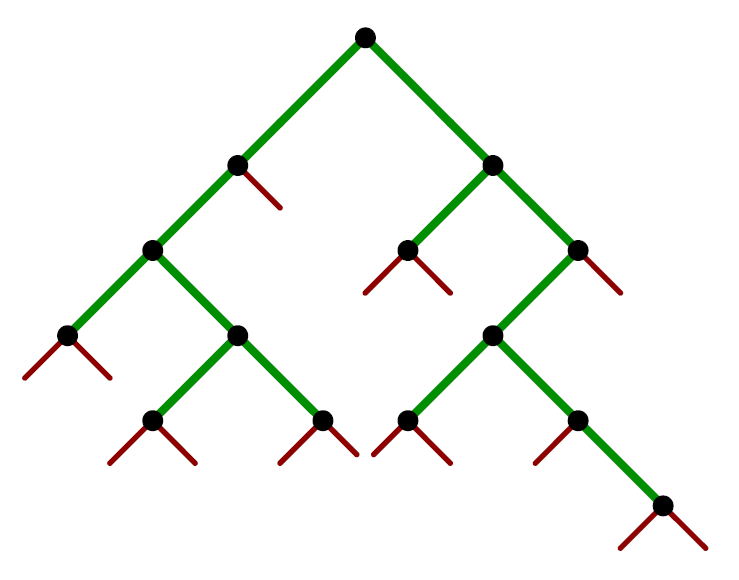
\includegraphics[width=0.5\linewidth]{images/full-binary-3.png}
    \caption{Full binary tree for the (non-full) binary tree given in fig~\ref{fig:bt-fbt-attempt1}. Notice that all the leaf nodes are added during transformation}
    \label{fig:binary-to-full-solution}
\end{figure}
We can see that this solution addresses the issue in the first attempt. Intuitively because of following argument: in the previous attempt the problem was that given a full binary tree, it was hard to decide if a leaf node was originally present in the binary tree or added during transformation. Now, in the current solution, this issue does not arise, because for any leaf node originally present in the binary tree, we add two new leaves as its children. Thus, it can be observed that all the leaf nodes (and only these nodes) are added during transformation.

To see that this translation is well-defined, we can see that the transformed tree is full binary tree by construction itself. Surjectivity is also easy to prove. To recover a binary tree from any given full binary tree, simply remove all the leaf nodes. We discussed injection informally. To give a formal argument, we first need to identify how to characterize two different binary trees? One of the hint as given during the discussion is to assign address to the nodes in the form of binary string, where 0-1 represents left or right child. 

Here we argued the bijection only intuitively and there are many things to be worked out formally. For example, proof for injection is not formally argued. Also, to argue surjection, we need to fix the number of nodes in full binary tree. Once we figure out this number, the argument for transformation being  well-defined also need to take that into account.

Writing a complete formal proof of bijection is left as homework exercise.

\paragraph{Bijection between plane trees and full binary trees}
A plane tree is a rooted tree with an ordering among the children. A plane tree can have more than two children. Figure~\ref{fig:plane-tree-1} shows a plane tree. 

\begin{figure}[h!]
    \centering
    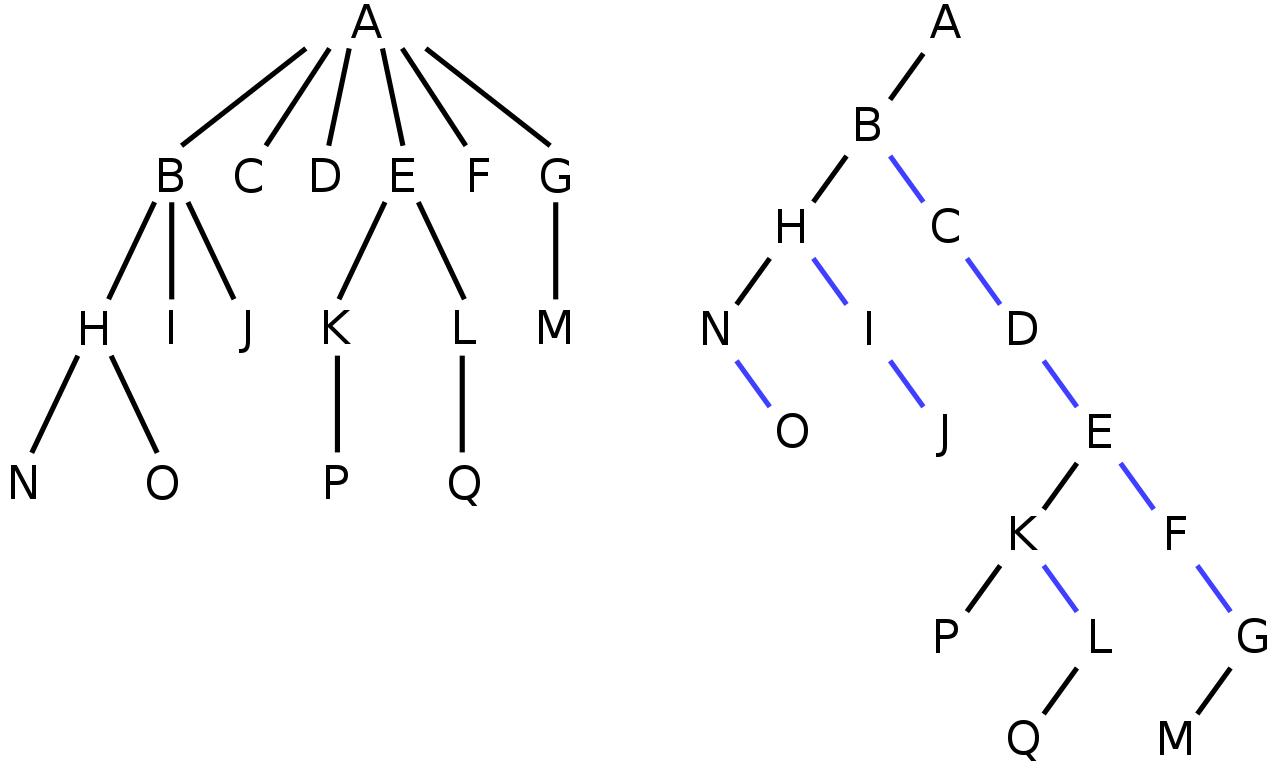
\includegraphics[width=0.8\linewidth]{images/plane-tree.png}
    \caption{An example of plane trees and its transformation to a binary tree}
    \label{fig:plane-tree-1}
\end{figure}

We are interested in studying the connection between plane trees and binary trees. The number of plane trees with $n$ nodes is equal to the number of binary trees with $n$ nodes. Thus, there is bijection between set of plane trees with $n$ nodes and the set of  binary trees with $n$ nodes. 

Here we define the bijection function. 

\noindent\underline{The Bijection:} Given any plane tree, do the following
\begin{itemize}
    \item For each node in the tree, 
    \begin{itemize}
        \item add its first child in plane tree as its left child in binary tree
        \item add its immediate sibling on right as its right child in binary tree.
    \end{itemize} child in the binary tree.
\end{itemize}
By following the above rule, we get a binary tree from given plane tree.

Observe that in the binary tree thus obtained, root node has only one child, while in general, in a binary tree the root can have both its children. Hence, we won't include the root as part of the binary tree.

Writing formal argument for all the properties is left as homework excercise.
